\chapter{Results}
In this chapter we examine the rendered output results of our implementation of our BRDF models applied to different input patches such as the Blaze grating and the Elaphe $\ref{fig:elpahespecies}$ and Xenopeltis $\ref{fig:xenospeicies}$ snake skins nanostructures. We are discussing and comparing both, their BRDF maps $\ref{fig:brdfmapexplanation}$ and the corresponding renderings on a snake geometry as shown in section $\ref{sec:snakegeomrenderings}$, for various input parameters. Last we also show a real experimental image showing the effect of diffraction for setting readers perception about expected results.

\section{BRDF maps}
A BRDF map shows a shader's output for all possible viewing directions for a given fixed, incident light direction. We assume that each viewing direction is expressed in spherical coordinates (See appendix $\ref{sec:sphericalcoordinates}$) $(\theta_v, \phi_v)$ and is represented in the map at a point 

\begin{align}
(x,y) = (sin(\theta_v)cos(\phi_v), sin(\theta_v)sin(\phi_v))
\end{align}

with its origin at the center of the map. The light direction for normal incidence $(\theta_i, \phi_i)$ has been fixed to $(0,0)$ for our rendered results.

\begin{figure}[H]
  \centering
  \subfigure[BRDF map schema]{
    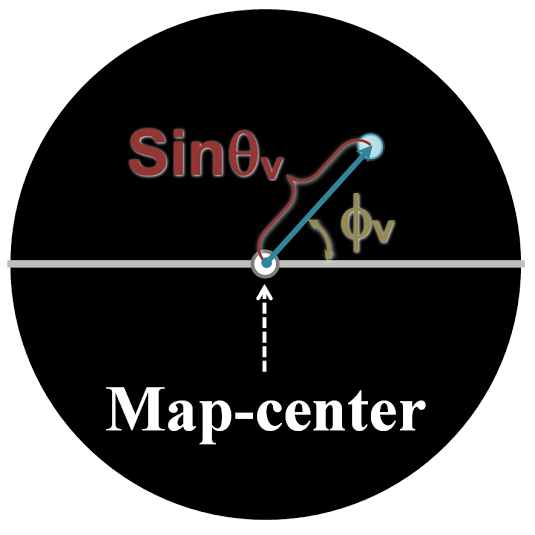
\includegraphics[scale=0.3]{resultsnew/brdfmapschema.png}
    \label{fig:brdfmapschema}
  }
~
  \subfigure[Light reflection geometrical setup]{
    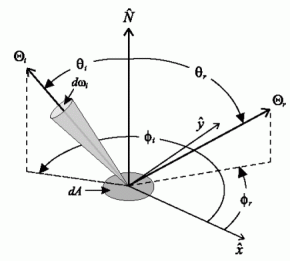
\includegraphics[scale=1.05]{results/Lightreflectiongeometry.png}
    \label{fig:lightreflectiongeometry}
  }
~

\caption[BRDF Map]{BRDF maps$\footnotemark$ for different patches: $\Theta=(\theta_i,\phi_i)$ is the direction of light propagation}
\label{fig:brdfmapexplanation}
\end{figure}
\footnotetext{image source of figure:
\begin{itemize}
  \item \ref{fig:brdfmapschema}: Taken from D.S.Dhillon et al's Paper $\cite{daljitpaper}$
  \item \ref{fig:lightreflectiongeometry}: Taken from \texttt{http://math.nist.gov/\textasciitilde FHunt/appearance/brdf.html}
  \end{itemize}
}

%%TODO maybe add glue fun - refere to schematics.
%%TODO say something about used gratings.

\begin{figure}[H]
  \centering
  \subfigure[Blaze grating with scale of 2.500 $\mu m$]{
    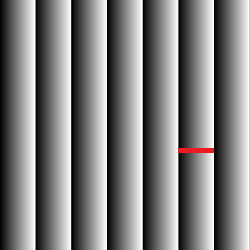
\includegraphics[scale=0.5]{evaluation/blaze_res.png}
    \label{fig:blazegratingpatch}
  }
~
  \subfigure[Elaphe patch with scale of 3.270 $\mu m$]{
    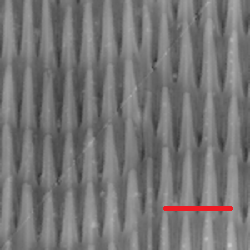
\includegraphics[scale=0.5]{evaluation/elaphe_res.png}
    \label{fig:elpahegratingpatch}
  }
~
  \subfigure[Xenopeltis patch with scale of 3.210 $\mu m$]{
    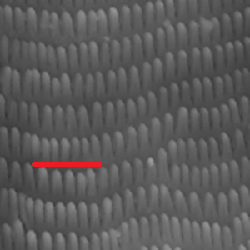
\includegraphics[scale=0.5]{evaluation/xeno_res.png}
    \label{fig:xenogratingpatch}
  }

\caption[Our Diffraction Gratings]{Cutouts of our nano-scaled surface gratings used for rendering with actual our shader with a scale indicator (red line) for each patch. Note that for actual rendering, we use larger patches.}
\label{fig:gratingpatches}
\end{figure}

Figure $\ref{fig:brdfmapsdiffpatches}$ shows the BRDF maps of the full lambda space sampling approach (\textbf{FLSS}) as described in section $\ref{sec:fragmentshader}$ applied on different nanoscale surface gratings shown in figure $\ref{fig:gratingpatches}$. In subfigure $\ref{fig:brdfmapBlaze}$ we see the BRDF map for the Blazed grating, showing high relative brightness for its first order diffraction, i.e. for the Blazed gratings most of the diffracted spectral energy lies in its first order. Notice that the surface of blazed grating is forming a step structure for which the angle between the step normal and the grating normal is denoted by $\emph{blaze angle}$. Every blazed grating is manufactred in the Littrow$\footnote{For further information please see \texttt{http://en.wikipedia.org/wiki/Blazed\textunderscore grating}.}$ configuration. This means that the blaze angle is chosen such that for a chosen mode m and a chosen wavelength $\lambda$ with maximum intensity and the incidence angle are identical. Thus a blazed grating has its maximal efficiency for the choosen wavelength of the light. Higher diffraction modes are still perceivable (second and higher diffraction orders) but with a much lower relative brightness. The asymmetry in the brigthness of the pattern is due to the asymmetric geometry of the grating $\ref{fig:blazegratingpatch}$. \\

The finger-like structures contained in the Elaphe surface grating $\ref{fig:elpahegratingpatch}$ are considerably regularly aligned and hence diffraction occurs along the horizontal axis for the BRDF map as shown in figure $\ref{fig:brdfmapElaphe}$. The reason for not seeing any strong diffraction color contribution along other directions in the BRDF map is due to the fact that these ‘nano-fingers’ overlap across layers and thus do not exhibit any well-formed periodicity along finger direction. \\

For the Xenopeltis surface grating shown in figure $\ref{fig:xenogratingpatch}$, we observe diffraction along many different, almost vertical directions in the BRDF map $\ref{fig:brdfmapXeno}$ since the layers of the finger-like structures do not overlap and are shifted significantly along their length but still exhibit some local consistency. A similar argument holds true for diffraction across locally periodic finger patches with slightly different orientations. 

\begin{figure}[H]
  \centering
  \subfigure[Blazed grating]{
    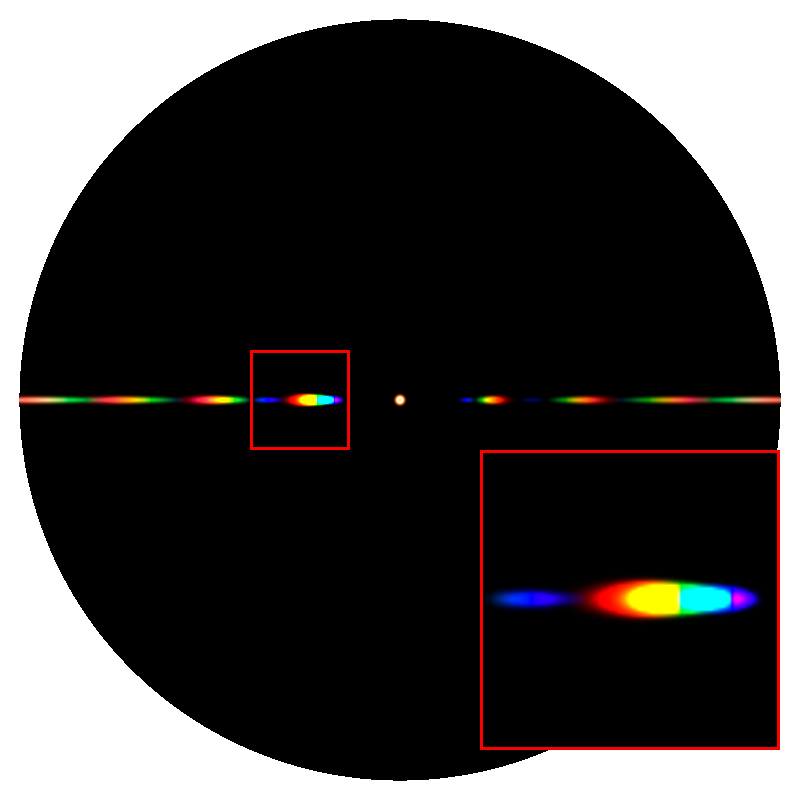
\includegraphics[scale=0.16]{nresults/brdfmaps/flss_gratings/blazed.png}
    \label{fig:brdfmapBlaze}
  }
~
  \subfigure[Elaphe grating]{
    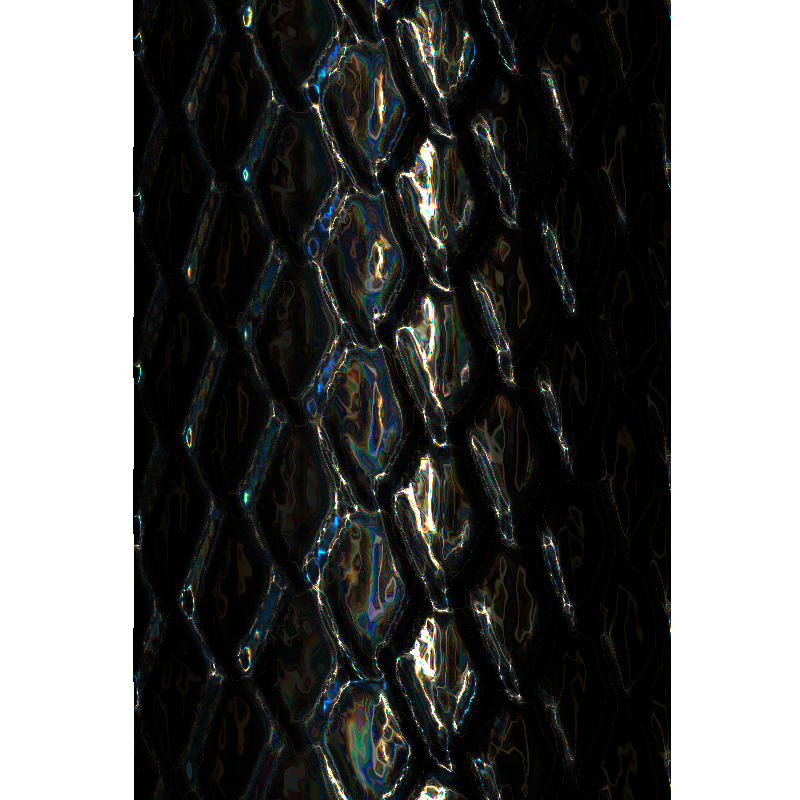
\includegraphics[scale=0.16]{nresults/brdfmaps/flss_gratings/elaphe.png}
    \label{fig:brdfmapElaphe}
  }
~
  \subfigure[Xenopeltis grating]{
    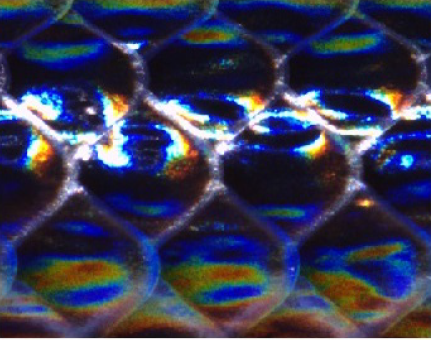
\includegraphics[scale=0.16]{nresults/brdfmaps/flss_gratings/xeno.png}
    \label{fig:brdfmapXeno}
  }

\caption[BRDF Map: FLSS Approach applied on various Gratings]{BRDF maps for different patches}
\label{fig:brdfmapsdiffpatches}
\end{figure}

%%TODO eplain what gound truth is refering to, what it is supposed to denote.

Figure $\ref{fig:brdfmapsdiffrenderingapproaches}$ shows BRDF maps of all our BRDF models applied on the Blaze grating. Figure $\ref{fig:brdfmapblazeallLambda}$ shows the FLSS shading approach result for our blazed grating and it is used in order to compare with our other rendering approaches. \\

Figure $\ref{fig:brdfmapblazeonlyreq}$ shows the BRDF map for the NMM approach, introduced in section $\ref{sec:nmmapproach}$, which is close to the FLSS approach as verified in section $\ref{sec:approachesverifications}$ (see figure $\ref{fig:blazneval}$). Nevertheless there is a small, noticeable difference: For the NMM approach we see a white, circular spot around the map center. Nevertheless, apart from this white spot, the NMM approach resembles the FLSS approach. The reason for this differences is due to the fact that the NMM approach treats the center of a BRDF map as a special case, as described in section $\ref{sec:nmmapproach}$. Technically, every location around a small $\epsilon$-circumference from the map center gets white color assigned. \\

Figure $\ref{fig:brdfmapblazepq}$ shows the BRDF map for the PQ approach which relies on sinc-interpolation. The PQ BRDF map and the FLSS results are visual alike. In contrast to the evaluation plots in figure $\ref{fig:evaluationdiffshaderpq}$, the BRDF map for the PQ approach matches well woth the one for the FLSS approach. Compared to FLSS, one difference we notice is that the first order of diffraction is a little spread for the PQ approach. \\

Last, let us consider figure $\ref{fig:brdfmapblazegem}$ which shows the BRDF map produced by using Nvidia Gem's implementation $\cite{cpugems}$ of Stam's BRDF model corresponding to periodic like structures with regularily repeated bumps (along y-axis of the BRDF map). This corresponds to a one dimensional diffraction grating, along the x-axis. This model only uses the spacing $d$ of a given grating. It also always produces highly symmetric results and fails to confirm with the Littrow configuration.   

% brdf maps patches
\begin{figure}[H]
  \centering
  \subfigure[FLSS]{
    \includegraphics[scale=0.25]{nresults/brdfmaps/approaches_blazed/flss.png}
    \label{fig:brdfmapblazeallLambda}
  }
~
  \subfigure[NMMS]{
    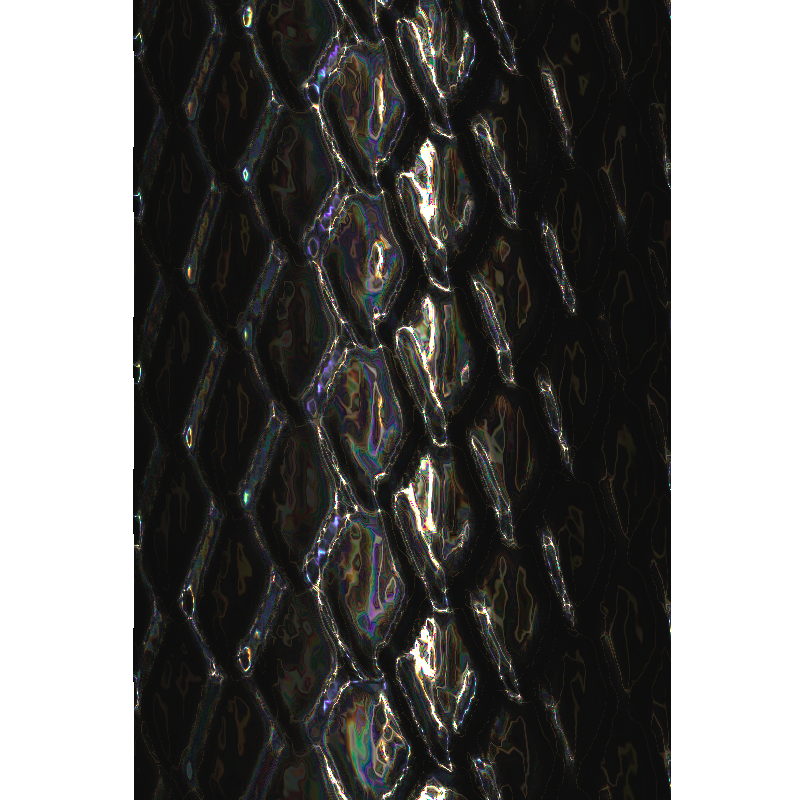
\includegraphics[scale=0.25]{nresults/brdfmaps/approaches_blazed/nmm.png}
    \label{fig:brdfmapblazeonlyreq}
  }

  \subfigure[PQ]{
    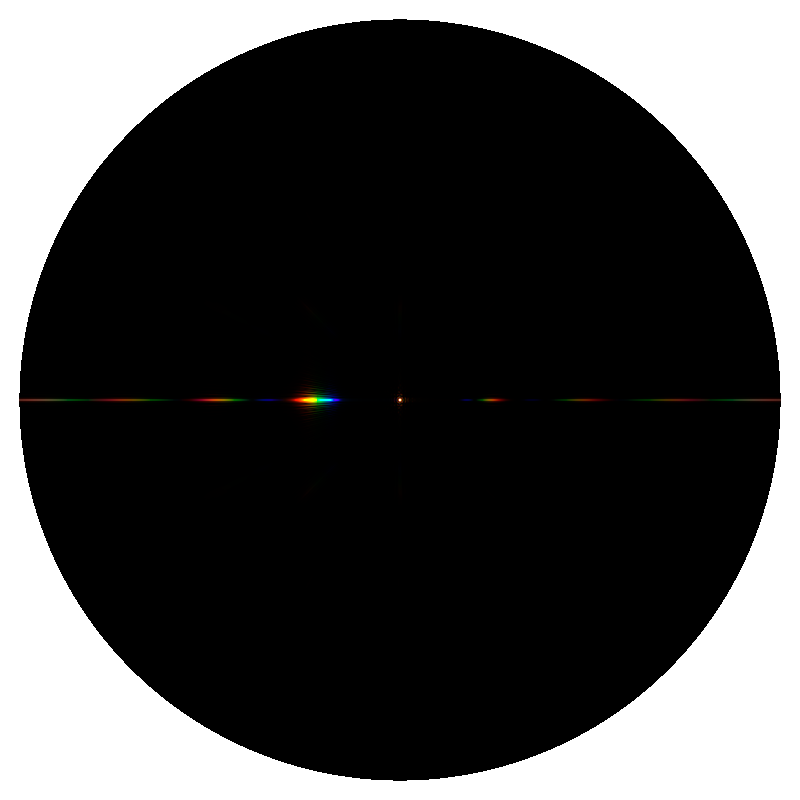
\includegraphics[scale=0.25]{nresults/brdfmaps/approaches_blazed/pqsinc.png}
    \label{fig:brdfmapblazepq}
  }
~
  \subfigure[Nvidia Gem]{
    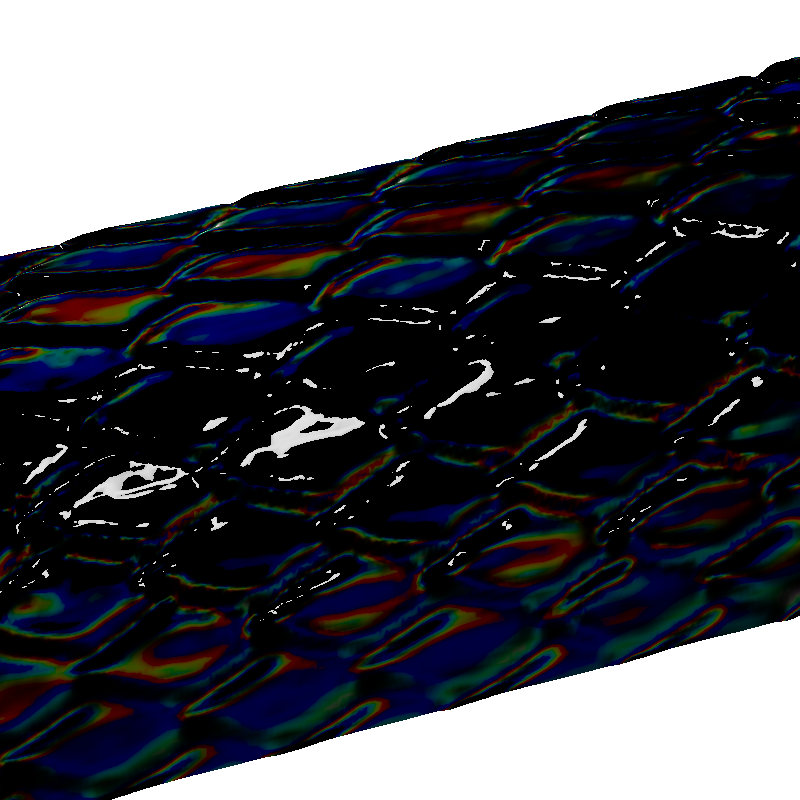
\includegraphics[scale=0.25]{nresults/brdfmaps/approaches_blazed/gem.png}
    \label{fig:brdfmapblazegem}
  }
    
\caption[BRDF Map: Our Approaches applied on a Blazed Grating]{BRDF maps for Blazed grating comparing our different rendering approaches}
\label{fig:brdfmapsdiffrenderingapproaches}
\end{figure}

Figure $\ref{fig:brdfmapsdifflambdastepsblaze}$ and figure $\ref{fig:brdfmapsdifflambdastepselaphe65}$ show the BRDF maps for different wavelength step sizes used in the fragment shader for the FLSS approach applied to the blazed grating and the Elaphe snake shed, respectively. Within our fragment shaders the outermost loop iterates over the range $[380nm, 780nm]$ for a given step size $\lambda_{step}$ to integrate over the wavelength spectrum as illustrated in algorithm $\ref{alg:fragmentshaderall}$. Having bigger step sizes implies having fewer $\lambda$-samples which will reduce the overall runtime of a shader but it will also introduce artifacts and therefore lower the overall shading quality. For an Elaphe surface grating, artifacts are perceivable when $\lambda_{step} \geq 10nm$. Results produced by using $5nm$ step sizes do not differ from those produced by using $\lambda_{step}= 1nm$. This allows us to set $\lambda_{step}$ at $5nm$. For a Blazed grating we may chose even bigger step sized without losing any rendering quality(see figure $\ref{fig:brdfmapsdifflambdastepsblaze}$).   

\begin{figure}[H]
  \centering
  \subfigure[$\lambda_{step=1 nm}$]{
    \includegraphics[scale=0.16]{nresults/brdfmaps/flss_blazed_lambdasteps/1.png}
    \label{fig:brdfmapsDiffLambdaStepsL1Blaze}
  }
~
  \subfigure[$\lambda_{step=5 nm}$]{
    \includegraphics[scale=0.16]{nresults/brdfmaps/flss_blazed_lambdasteps/5.png}
    \label{fig:brdfmapsDiffLambdaStepsL5Blaze}
  }
~
  \subfigure[$\lambda_{step=10 nm}$]{
    \includegraphics[scale=0.16]{nresults/brdfmaps/flss_blazed_lambdasteps/10.png}
    \label{fig:brdfmapsDiffLambdaStepsL10Blaze}
  }
  
  \subfigure[$\lambda_{step=25 nm}$]{
    \includegraphics[scale=0.16]{nresults/brdfmaps/flss_blazed_lambdasteps/25.png}
    \label{fig:brdfmapsDiffLambdaStepsL25Blaze}
  }
~
  \subfigure[$\lambda_{step=50 nm}$]{
    \includegraphics[scale=0.16]{nresults/brdfmaps/flss_blazed_lambdasteps/50.png}
    \label{fig:brdfmapsDiffLambdaStepsL50Blaze}
  }
~ 
  \subfigure[$\lambda_{step=100 nm}$]{
    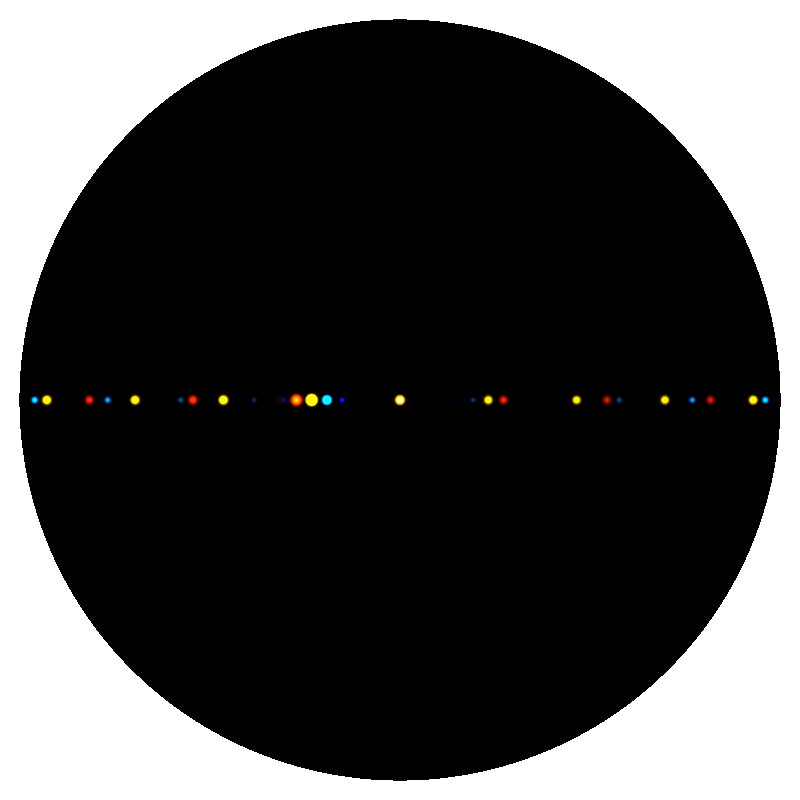
\includegraphics[scale=0.16]{nresults/brdfmaps/flss_blazed_lambdasteps/100.png}
    \label{fig:brdfmapsDiffLambdaStepsL100Blaze}
  }
  
\caption[BRDF Map: Varying step sizes FLSS Blazed Grating]{Blazed grating at $2.5 \mu m$: Different $\lambda$ step sizes}
\label{fig:brdfmapsdifflambdastepsblaze}
\end{figure}

% elpahe steps
\begin{figure}[H]
  \centering
  \subfigure[$\lambda_{step=1 nm}$]{
    \includegraphics[scale=0.43]{nresults/brdfmaps/flss_elaphe_lambdasteps/1.png}
    \label{fig:brdfmapsDiffLambdaStepsL1Elaphe65}
  }
~
  \subfigure[$\lambda_{step=5 nm}$]{
    \includegraphics[scale=0.43]{nresults/brdfmaps/flss_elaphe_lambdasteps/5.png}
    \label{fig:brdfmapsDiffLambdaStepsL5Elaphe65}
  }
~
  \subfigure[$\lambda_{step=10 nm}$]{
    \includegraphics[scale=0.43]{nresults/brdfmaps/flss_elaphe_lambdasteps/10.png}
    \label{fig:brdfmapsDiffLambdaStepsL10Elaphe65}
  }
  
  \subfigure[$\lambda_{step=25 nm}$]{
    \includegraphics[scale=0.43]{nresults/brdfmaps/flss_elaphe_lambdasteps/25.png}
    \label{fig:brdfmapsDiffLambdaStepsL25Elaphe65}
  }
~
  \subfigure[$\lambda_{step=50 nm}$]{
    \includegraphics[scale=0.43]{nresults/brdfmaps/flss_elaphe_lambdasteps/50.png}
    \label{fig:brdfmapsDiffLambdaStepsL50Elaphe65}
  }
~ 
  
\caption[BRDF Map: Varying step sizes FLSS Elaphe Grating]{Elaphe grating at $65 \mu m$: Different $\lambda$ step sizes}
\label{fig:brdfmapsdifflambdastepselaphe65}
\end{figure}

The figures $\ref{fig:pqblaze}$, $\ref{fig:pqelaphe}$, $\ref{fig:pqxeno}$ show a comparison of the BRDF maps produced by the FLSS approach (on the left) and the PQ shading approach (on the right) applied on all our patches. For Blazed grating, as already mentioned, we notice that both approaches, FLSS and PQ, look similar but have notable differences. In the PQ map, the first order diffraction color contribution is spread. In genral, a Blazed Grating is manufactured in a way that a large fraction of the incident light is diffracted preferentially into the first order. Therefore, most of the energy in its BRDF map lies in the first order of diffraction at its blaze angle. This implies that largest portion of the color contribution, visible on the corresponding BRDF map, lies at that angle. In figure $\ref{fig:pqblaze}$, in contrast to the results produced by the FLSS approach, we see color fringes at the first order modes in the BRDF map produced by our PQ approach. This implies that the PQ approach does not produce reliable results which also affirms our evaluation plots shown in figure $\ref{fig:evaluationdiffshaderpq}$. The BRDF resulting BRDF mapf for the Elaphe and Xenopeltis gratings using the PQ approach are similar to those resulting by the FLSS approach. Nevertheless they also exhibit some artifacts, similar to these discussed for the Blazed grating.

\begin{figure}[H]
  \centering
  \subfigure[FLSS Approach: Blazed grating]{
    \includegraphics[scale=0.25]{nresults/brdfmaps/approaches_blazed/flss.png}
    \label{fig:fullLambdaBlaze}
  }
~
  \subfigure[PQ Sinc Interpolation Approach: Blazed grating]{
    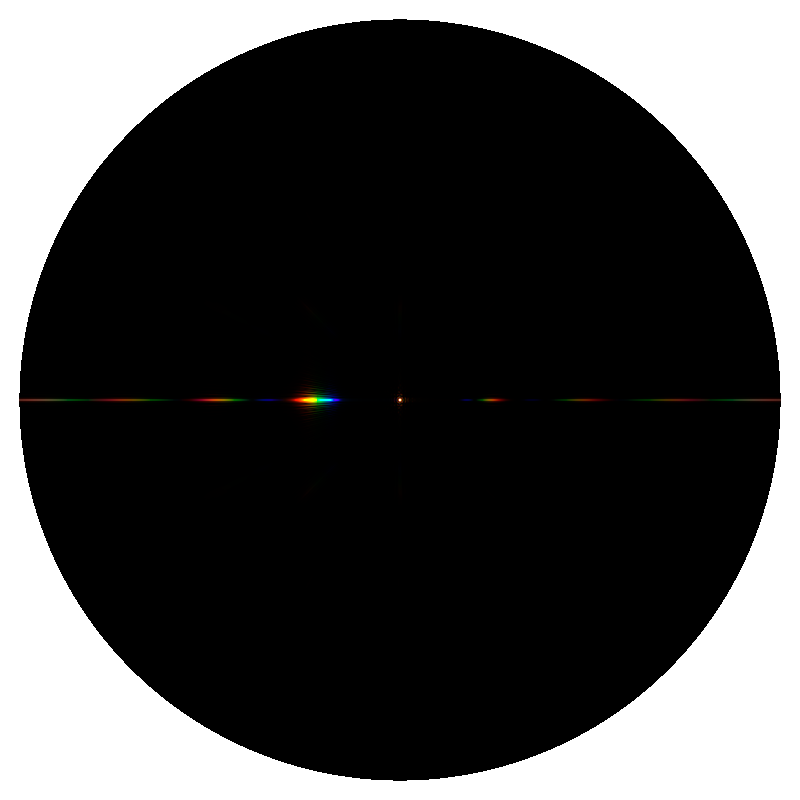
\includegraphics[scale=0.25]{nresults/brdfmaps/approaches_blazed/pqsinc.png}
    \label{fig:pqBlaze}
  }
\caption[BRDF Map: PQ vs FLSS Approach on Blazed Grating]{A comparison between the PQ- and the FLSS approach applied on an Blazed grating.}
\label{fig:pqblaze}
\end{figure}

\begin{figure}[H]
  \centering
  \subfigure[FLSS Approach: Elaphe grating]{
    \includegraphics[scale=0.25]{nresults/brdfmaps/flss_pq_elaphe/flss.png}
    \label{fig:fullLambdaElaphe}
  }
~
  \subfigure[PQ Approach: Elaphe grating]{
    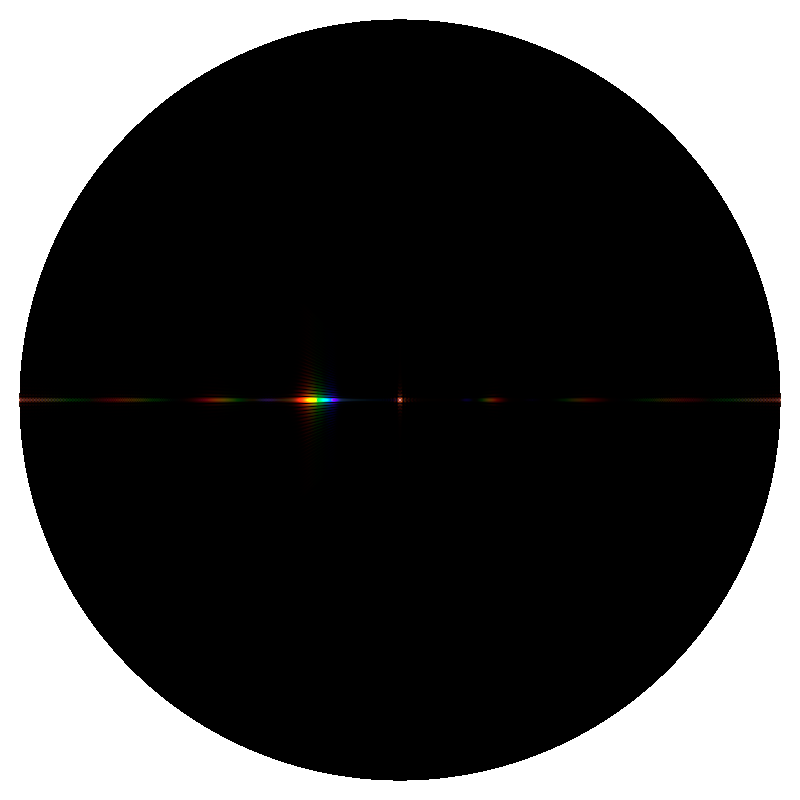
\includegraphics[scale=0.25]{nresults/brdfmaps/flss_pq_elaphe/pq.png}
    \label{fig:pqElaphe}
  }

\caption[BRDF Map: PQ vs FLSS Approach on Elaphe Grating]{A comparison between the PQ- and the FLSS approach applied on an Elaphe grating.}
\label{fig:pqelaphe}
\end{figure}

\begin{figure}[H]
  \centering
  \subfigure[FLSS Approach: Xenopeltis grating $\theta_i = 0 \degree$]{
    \includegraphics[scale=0.19]{nresults/brdfmaps/flss_xeno_thetai/0.png}
    \label{fig:fullLambdaXenoti0}
  }
~
  \subfigure[PQ Approach: Xenopeltis grating $\theta_i = 0 \degree$]{
    \includegraphics[scale=0.19]{nresults/brdfmaps/pq_xeno_thetai/0.png}
    \label{fig:pqXenoti0}
  }

  \subfigure[FLSS Approach: Xenopeltis grating $\theta_i = 10 \degree$]{
    \includegraphics[scale=0.19]{nresults/brdfmaps/flss_xeno_thetai/10.png}
    \label{fig:fullLambdaXenoti10}
  }
~
  \subfigure[PQ Approach: Xenopeltis grating $\theta_i = 10 \degree$]{
    \includegraphics[scale=0.19]{nresults/brdfmaps/pq_xeno_thetai/10.png}
    \label{fig:pqXenoti10}
  }
  
  \subfigure[FLSS Approach: Xenopeltis grating $\theta_i = 20 \degree $]{
    \includegraphics[scale=0.19]{nresults/brdfmaps/flss_xeno_thetai/20.png}
    \label{fig:fullLambdaXenoti20}
  }
~
  \subfigure[PQ Approach: Xenopeltis grating $\theta_i = 20 \degree $]{
    \includegraphics[scale=0.19]{nresults/brdfmaps/pq_xeno_thetai/20.png}
    \label{fig:pqXenoti20}
  }
  
\caption[BRDF Map: PQ vs FLSS Approach on Xenopeltis Grating]{A comparison between the PQ- and the FLSS approach applied on an Xenopeltis grating.}
\label{fig:pqxeno}
\end{figure}

Figure $\ref{fig:brdfmapsdiffsigmasizeblaze}$ shows BRDF maps for the FLSS approach when applied to the Blazed grating, while varying the value for the spatial variance $\sigma_s$ for the coherence window. This is akin to changing the coherence length for the incident light. We see that the lower the coherence length gets, the fewer of the interacting grating periods are involved. Having fewer periods cause the production of overlapping blurry diffraction bands (i.e. blobs, see e.g. figure $\ref{fig:brdfmapsDiffSigmaStepsL5Blaze}$) for different wavelengths $\lambda$. Thus, when reducing the number of periods this will produces blurry artifiacts which ends in having poorly resolved colors.  

\begin{figure}[H]
  \centering
  \subfigure[$\sigma_{s=3.25 \mu m}$]{
    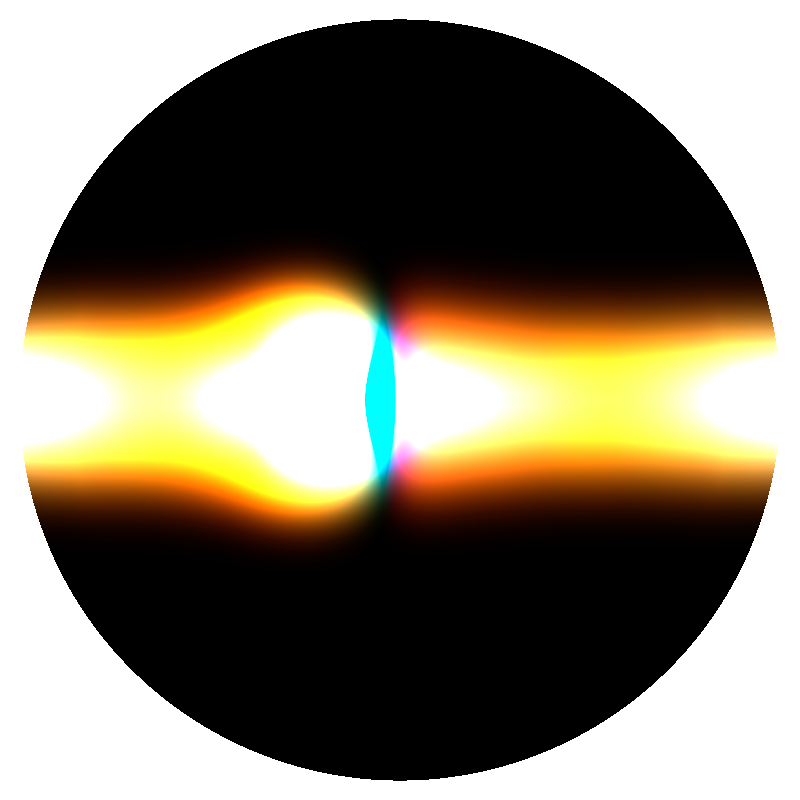
\includegraphics[scale=0.16]{nresults/brdfmaps/flss_blazed_sigmas/3_25.png}
    \label{fig:brdfmapsDiffSigmaStepsL1Blaze}
  }
~
  \subfigure[$\sigma_{s=6.5 \mu m}$]{
    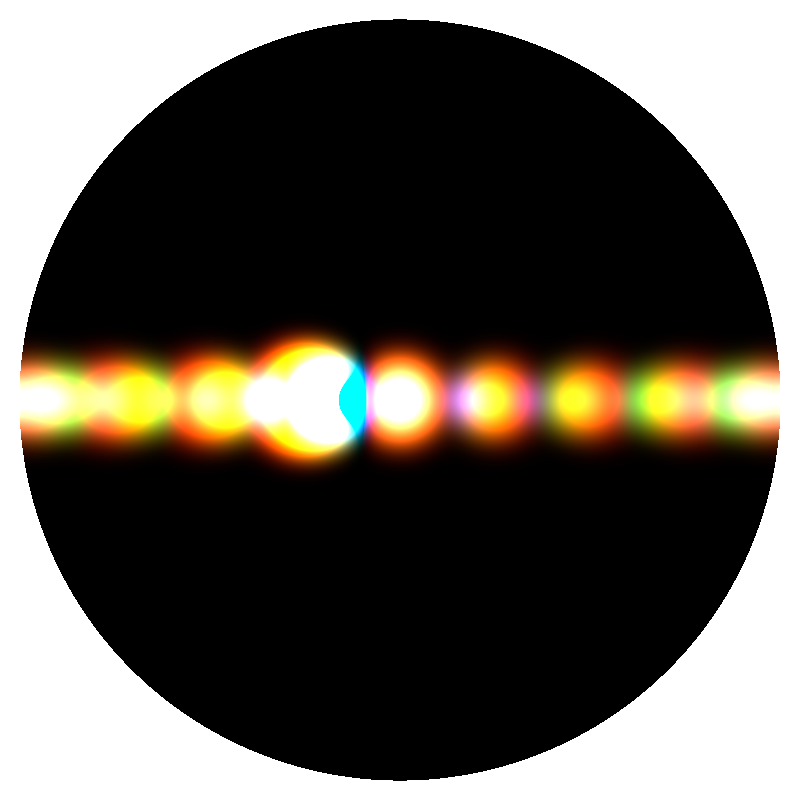
\includegraphics[scale=0.16]{nresults/brdfmaps/flss_blazed_sigmas/6_5.png}
    \label{fig:brdfmapsDiffSigmaStepsL5Blaze}
  }
~
  \subfigure[$\sigma_{s=15 \mu m}$]{
    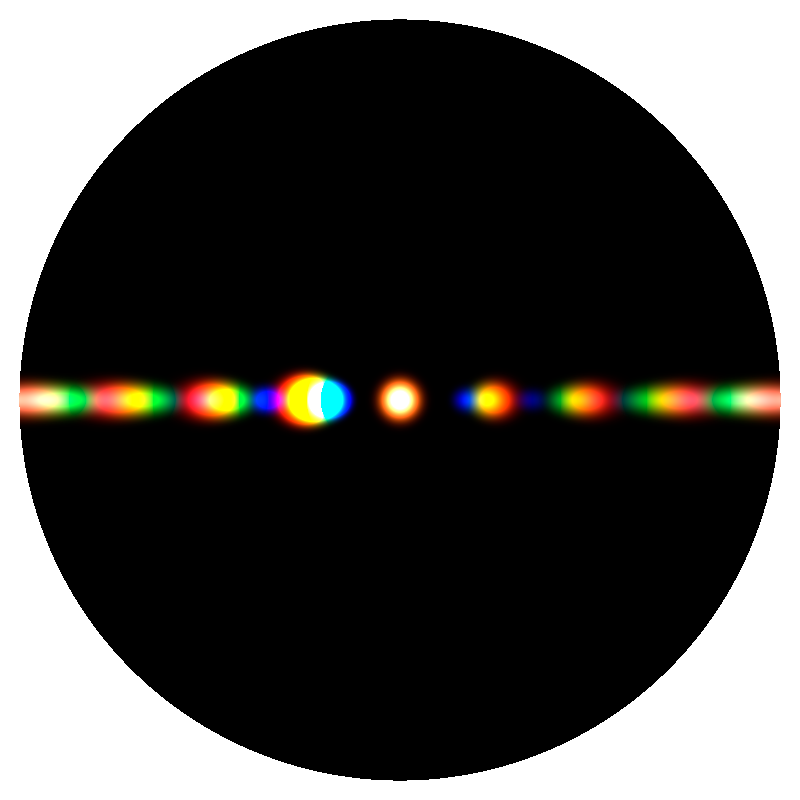
\includegraphics[scale=0.16]{nresults/brdfmaps/flss_blazed_sigmas/15.png}
    \label{fig:brdfmapsDiffSigmaStepsL10Blaze}
  }
  
  \subfigure[$\sigma_{s=30 \mu m}$]{
    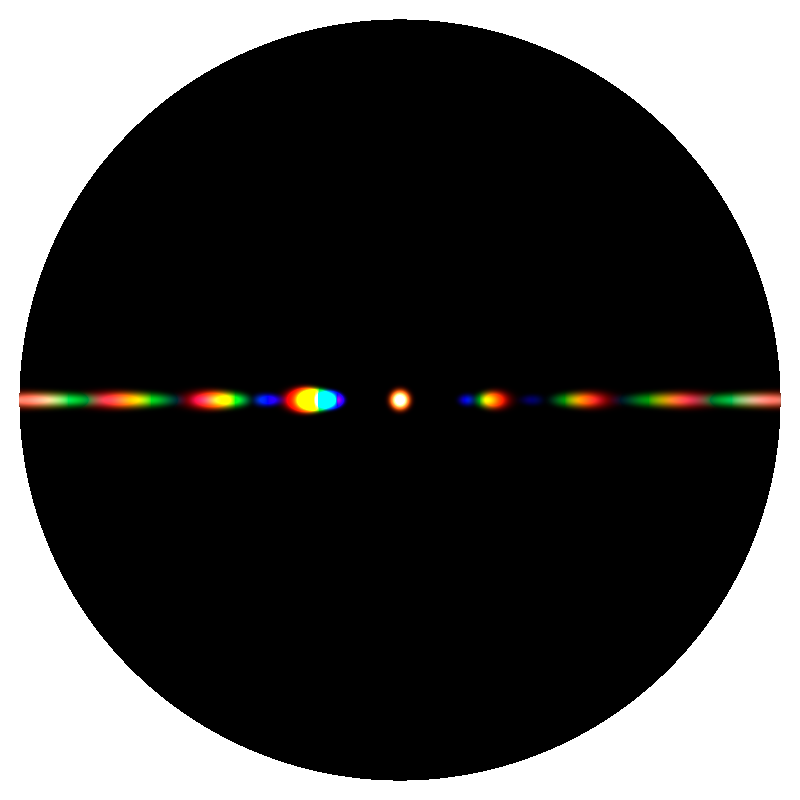
\includegraphics[scale=0.16]{nresults/brdfmaps/flss_blazed_sigmas/30.png}
    \label{fig:brdfmapsDiffSigmaStepsL25Blaze}
  }
~
  \subfigure[$\sigma_{s=45 \mu m}$]{
    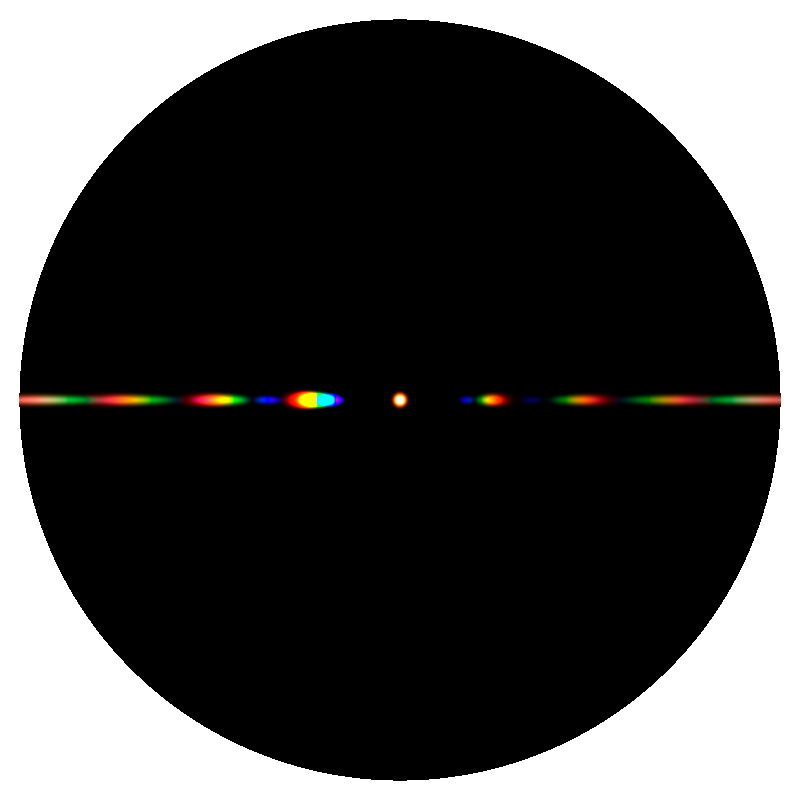
\includegraphics[scale=0.16]{nresults/brdfmaps/flss_blazed_sigmas/45.png}
    \label{fig:brdfmapsDiffSigmaStepsL50Blaze}
  }
~ 
  \subfigure[$\sigma_{s=65 \mu m}$]{
    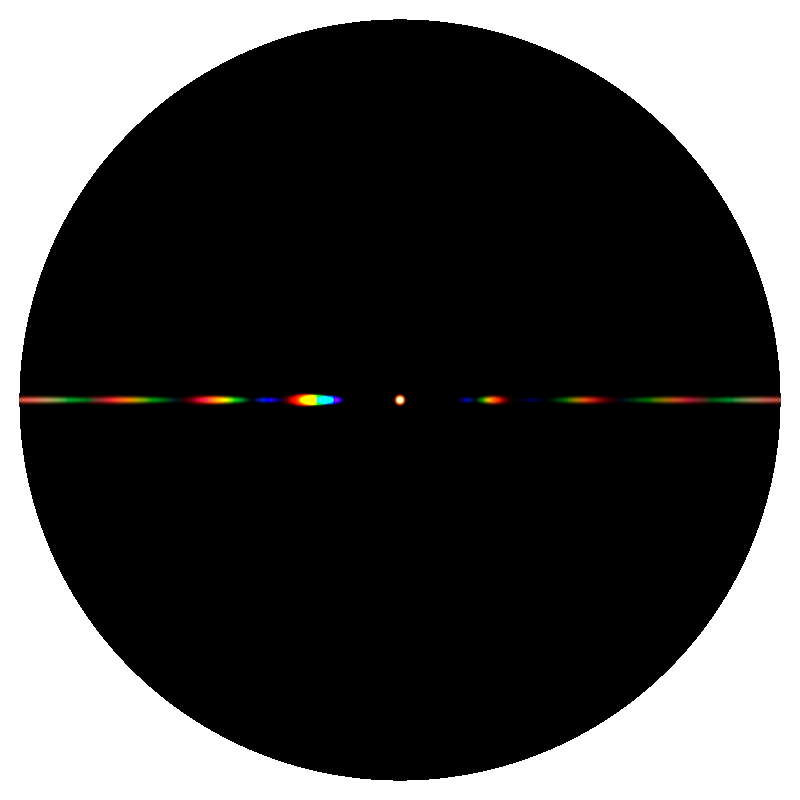
\includegraphics[scale=0.16]{nresults/brdfmaps/flss_blazed_sigmas/65.png}
    \label{fig:brdfmapsDiffSigmaStepsL100Blaze}
  }
  
\caption[BRDF Map: Different spatial variance $\sigma_s$ values]{Blazed grating with periodicity of $2.5 \mu m$: Different $\sigma_s$}
\label{fig:brdfmapsdiffsigmasizeblaze}
\end{figure}

Figures $\ref{fig:brdfmapstayloriterationsblaze}$ and $\ref{fig:brdfmapstayloriterationselaphe65}$ show the BRDF maps for the FLSS approach using a different number of terms $N$ used in the Taylor series approximation. For both input patches we clearly, visually observe the convergence of the taylor series for higher values of N. We visually observe convergence of the Taylor series for all our patches for a very large value of $N$$\footnote{Using N equal to 40 lead to visual convergence for all our used gratings.}$. \\

As discussed in section $\ref{sec:taylorapproximation}$ there exists a certain value of $N$ for which our approach converges. For all our shading approaches, applied on our gratings, we visually observed a convergence of their BRDF maps when using $N \geq 39$ DFT terms. Furthermore, for a Blazed grating it suffices to use only $N \geq 7$ - and for an Elaphe grating only $N \geq 9$ DFT terms. Notice, that these numbers of required DFT terms were empirically determined with a trial and error strategy. \\

However, by making use of Taylor error term estimates, as introduced in the appendix section $\ref{chap:taylorseriesapproxappendix}$, we can derive an upper bound for $N$. This computation is dependent on many aspects, such as on the grating spacing, the sampling rate $dH$ and the used wavelenght spectrum. Thus, it is usually simpler to empirically determine an actual value for $N$ to be used. \\

In algorithm $\ref{alg:matlabprecomp}$ we compute different powers of DFT terms of our height fields $h$ by evaluating the expression $DFT(h)^n \cdot i^n$, where $i$ denotes the imaginary number $i$ and $n$ is a natural number. Note that when appliyng the DFT operator on a real or complex number (e.g. such as one particular value of our height field) we get a complex number. Using our Taylor series approximation has basically four possible convergence images, each having its own convergence radius. The reason for this is due to the fact we are multiplying the DFT terms by $i^n$. \\

In order to understand the reason behind this, let us consider the complex unit $i$. Raising $i$ to the power of a natural number $n$ leaves us four possible results as shown in equation $\ref{eq:thefourunits}$:
 
\begin{align}
  i^n = \left\{ \begin{array}{rl}
  1 &\mbox{ if $n \equiv_4 0$} \\
  i &\mbox{ if $n \equiv_4 1$} \\
  -1 &\mbox{ if $n \equiv_4 2$} \\
  -i &\mbox{ otherwise}
  \end{array} \right.
\label{eq:thefourunits}
\end{align}

Thus multiplying a complex number $c$, such as particular value of a DFT term, by $i$ raised to a certain power, will permute the the value of $c$.
Since we compute $\sum_{k=0}^N DFT(h)^k \cdot i^k$ we can split this summation into four partial summations, according to their applied power factor $i$. Each of these summands converges with a different convergence radius.

\begin{figure}[H]
  \centering
  \subfigure[$N=1$]{
    \includegraphics[scale=0.16]{nresults/brdfmaps/flss_xeno_taylor/0.png}
    \label{fig:brdfmapsTaylorN0Blaze}
  }
~
  \subfigure[$N=2$]{
    \includegraphics[scale=0.16]{nresults/brdfmaps/flss_xeno_taylor/1.png}
    \label{fig:brdfmapsTaylorN1Blaze}
  }
~
  \subfigure[$N=4$]{
    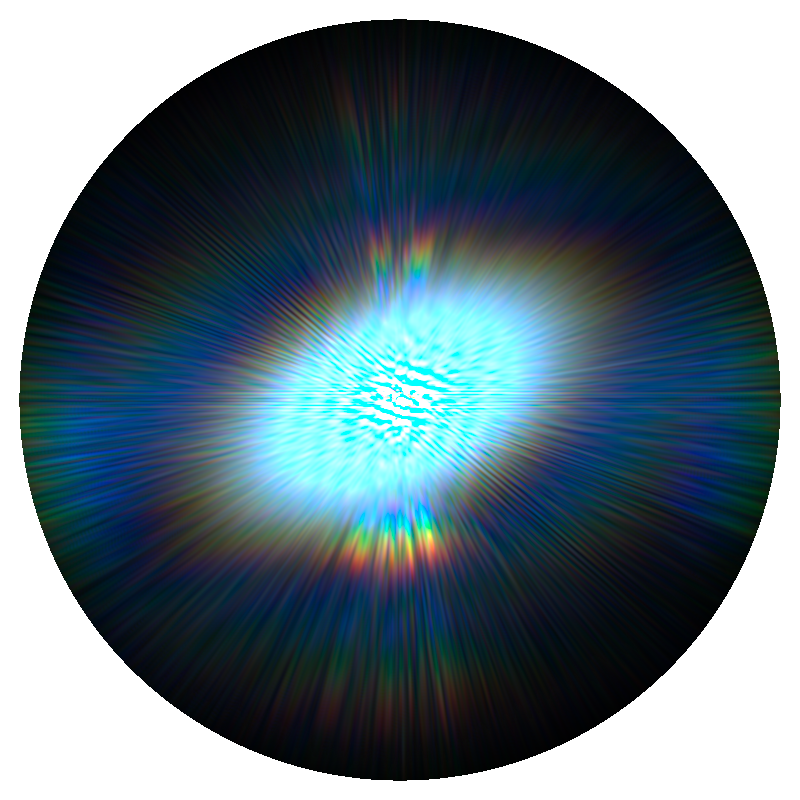
\includegraphics[scale=0.16]{nresults/brdfmaps/flss_xeno_taylor/3.png}
    \label{fig:brdfmapsTaylorN2Blaze}
  }
 
  \subfigure[$N=24$]{
    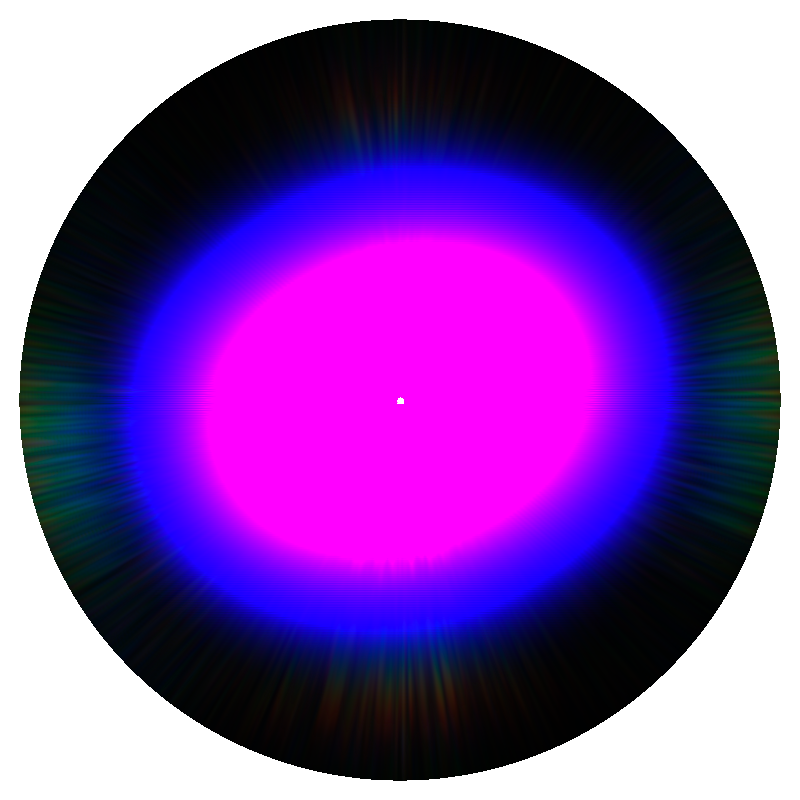
\includegraphics[scale=0.16]{nresults/brdfmaps/flss_xeno_taylor/23.png}
    \label{fig:brdfmapsTaylorN3Blaze}
  }
~
  \subfigure[$N=26$]{
    \includegraphics[scale=0.16]{nresults/brdfmaps/flss_xeno_taylor/25.png}
    \label{fig:brdfmapsTaylorN4Blaze}
  }
~
  \subfigure[$N=40$]{
    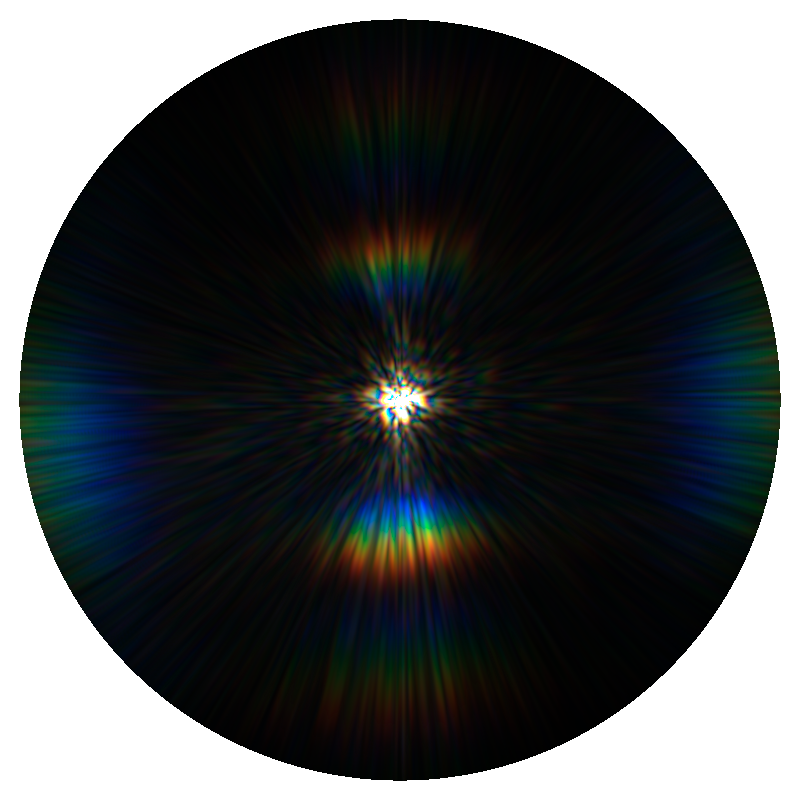
\includegraphics[scale=0.16]{nresults/brdfmaps/flss_xeno_taylor/39.png}
    \label{fig:brdfmapsTaylorN5Blaze}
  } 
  
\caption[BRDF Map: Xenopeltis Grating Convergence]{Blazed grating at $65 \mu m$: $N$ Taylor Iterations}
\label{fig:brdfmapstayloriterationsblaze}
\end{figure}

%taylor var elaphe
\begin{figure}[H]
  \centering
  \subfigure[$N=1$]{
    \includegraphics[scale=0.16]{nresults/brdfmaps/flss_elaphe_taylor/0.png}
    \label{fig:brdfmapsTaylorN0Elaphe65}
  }
~
  \subfigure[$N=2$]{
    \includegraphics[scale=0.16]{nresults/brdfmaps/flss_elaphe_taylor/1.png}
    \label{fig:brdfmapsTaylorN1Elaphe65}
  }
~
  \subfigure[$N=5$]{
    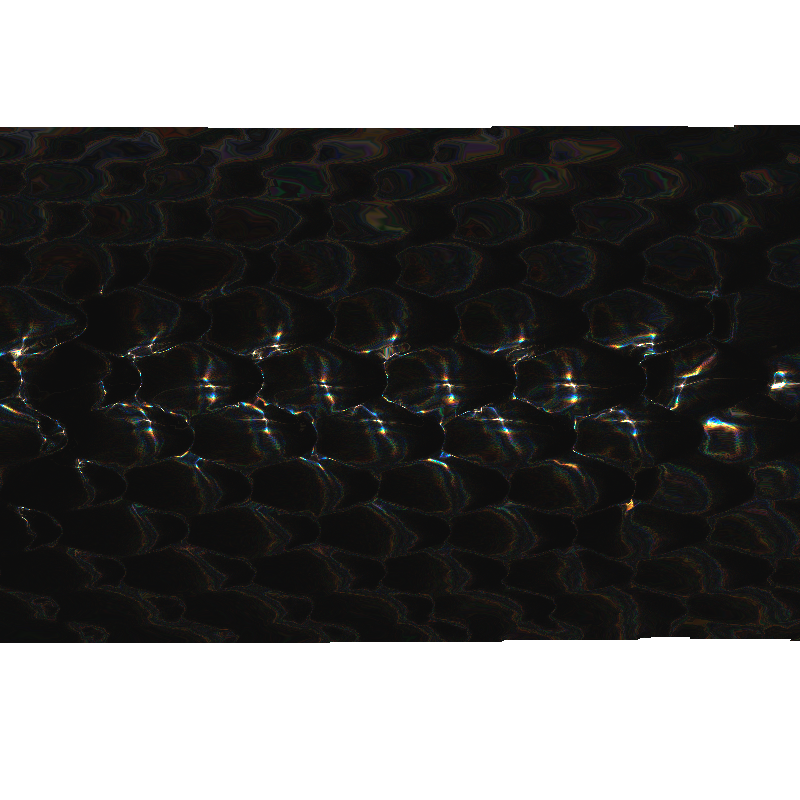
\includegraphics[scale=0.16]{nresults/brdfmaps/flss_elaphe_taylor/4.png}
    \label{fig:brdfmapsTaylorN2Elaphe65}
  }
  
  \subfigure[$N=10$]{
    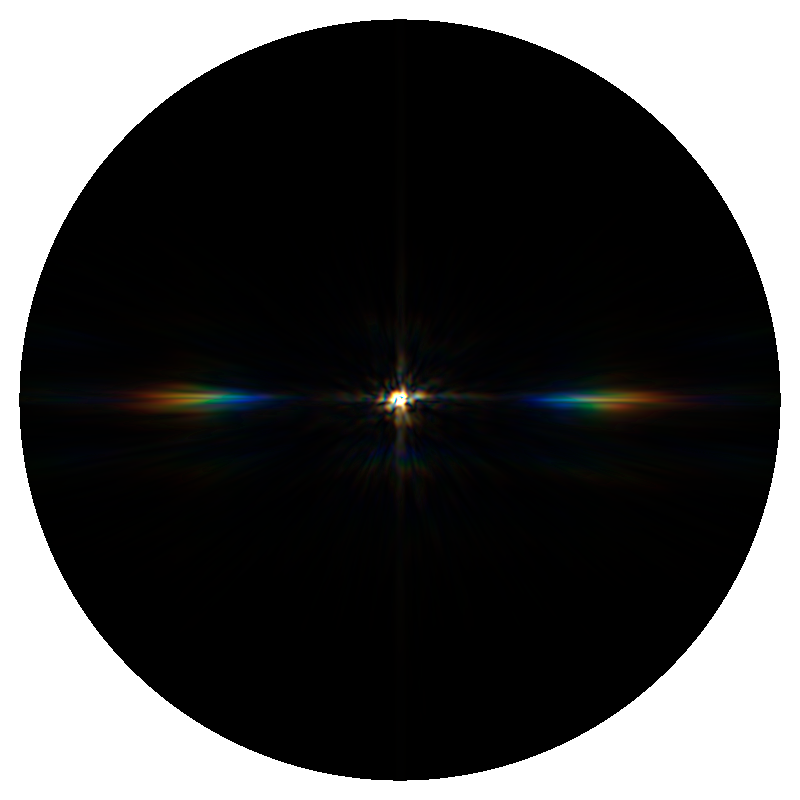
\includegraphics[scale=0.16]{nresults/brdfmaps/flss_elaphe_taylor/9.png}
    \label{fig:brdfmapsTaylorN3Elaphe65}
  }
~
  \subfigure[$N=11$]{
    \includegraphics[scale=0.16]{nresults/brdfmaps/flss_elaphe_taylor/10.png}
    \label{fig:brdfmapsTaylorN4Elaphe65}
  }
~
  \subfigure[$N=40$]{
    \includegraphics[scale=0.16]{nresults/brdfmaps/flss_elaphe_taylor/39.png}
    \label{fig:brdfmapsTaylorN5Elaphe65}
  }
  
\caption[BRDF Map: Elaphe Grating Convergence]{Elaphe grating at $65 \mu m$: $N$ Taylor Iterations}
\label{fig:brdfmapstayloriterationselaphe65}
\end{figure}

Figure $\ref{fig:brdfmapsxenodiffthetaiangles}$ shows the BRDF maps of the FLSS approach applied on the Xenopeltis snake shed, using different $\theta_i$ incident angles. When slightly moving the incident angle $\theta_i$, we can observe how the BRDF map changes. For higher values of $\theta_i$ we start seeing additional diffraction color contributions on the right side of the BRDF map. 

\begin{figure}[H]
  \centering
  \subfigure[Xenopeltis grating $\theta_i=0 \degree$]{
    \includegraphics[scale=0.15]{nresults/brdfmaps/flss_xeno_thetai/0.png}
    \label{fig:brdfmapXenoti0}
  }
~
  \subfigure[Xenopeltis grating $\theta_i=10 \degree$]{
    \includegraphics[scale=0.15]{nresults/brdfmaps/flss_xeno_thetai/10.png}
    \label{fig:brdfmapXenoti10}
  }
~
  \subfigure[Xenopeltis grating $\theta_i=20 \degree$]{
    \includegraphics[scale=0.15]{nresults/brdfmaps/flss_xeno_thetai/20.png}
    \label{fig:brdfmapXenoti20}
  }
  
\caption[BRDF Map: Varying Viewing Angles]{BRDF maps for Xenopeltis grating: different $\theta_i$ angles}
\label{fig:brdfmapsxenodiffthetaiangles}
\end{figure}

\section{Rendering Surface Geometries}
\label{sec:snakegeomrenderings}
In this section we are going to present our actual renderings simulating the effect of diffraction caused when a directional light source encounters different nano-scaled surfaces on a given curved snake mesh. We will see that diffraction colors change dramatically with changes in light direction, surface normals and viewing direction, which is typical for diffraction colors observed in nature. For rendering we are going to rely on our FLSS approach. Unfortunately, this approach is rather slow and can barely be considered as being interactively performing. Nevertheless, we have introduced some optimizations in order to make it interactive. \\

All rendered results shown in this section are produced by the FLSS approach since we have proven its validity in figure $\ref{fig:evaluationdiffshaderalllambda}$. Therefore, we can trust its renderings and may consider them as being accurate. Furthermore, as support of our evaluation plots regarding the NMM approach, that are shown in figure $\ref{fig:evaluationdiffshadernminmax}$, we also show results produced by the NMM approach. \\

The Laboratory of Artificial and Natural Evolution in Geneva provided us by a triangular mesh of a snake. This mesh was produced by a 3d scan of a Elaphe snake species and consists of 11696 vertices and 22950 faces. Note that, for all our renderings, we used this snake mesh. \\

Among all the snake species under consideration, their macroscopic geometry is highly similar. Only the geometry of their nano-structures varies and is responsible for a snake's iridescence. Thus, we can use the same snake surface model to render diffraction for different species. Table $\ref{tab:hardwarespecifications}$ lists the system specifications of the machine I used in order to produce the rendered images.

\begin{table}[H]
  \centering
  \begin{tabular}{|r|l|}
    \hline
    Processor & Intel i7 CPU 970 @ 3.20 GHz (12 CPUs) \\
    Memory & 12288 MB RAM \\
    Graphics Card & GeForce GTX 770 \\
    Graphics Clock & 1150 MHz \\
    Graphics Memory & 4096 MB \\
    Graphics Memory Bandwidth & 230.4 $GB/s$ MHz \\
    \hline  
  \end{tabular}
\caption[Hardware Specifications]{Hardware specifications of the machine used to render snake surface. Statistics are provided using the tool $\emph{NVIDIA Geforce Experience}$.}
\label{tab:hardwarespecifications}
\end{table}

Figure $\ref{fig:renderingdifferentsnankegratings}$ shows renderings produced by the FLSS approach applied on our snake mesh for different, given input patches. Due do the fact that a Blazed grating has its maximum intensity for a certain direction and the geometry of the snake mesh is curved i.e. is non-flat, we can expect rather less diffraction color contribution like shown in figure $\ref{fig:renderingelaphegrating}$. \\

%%TODO write something about similar configuration for blazed grating

In contrast, For both the renderings, we see colorful patterns on the skin of our snake species, Elaphe and Xenopeltis, due to the effect of diffraction. We see much less colorful patterns for Elaphe like shown in figure $\ref{fig:renderingelaphegrating}$ than for Xenopeltis like shown in figure $\ref{fig:renderingxenograting}$. This is consistent with the observations in the real world as shown in figure $\ref{fig:snakespecies}$. As observable figure $\ref{fig:elpahegratingpatch}$, the substructures (the finger like structures) in the height field of a Elaphe snake skin are not very regularly aligned along the y-axis. This is why the Elaphe species is less iridescent than the other specie. The Xenopeltis snake has a brownish body with no pigmentation, which makes the iridescence more spectacular than on Elaphe. 
 
\begin{figure}[H]
  \centering
  \subfigure[Blazed grating]{
    \includegraphics[scale=0.16]{nresults/snakerenderings/flss_gratings/blazed1552.png}
    \label{fig:renderingblazegrating}
  }
~
  \subfigure[Elaphe grating]{
    \includegraphics[scale=0.16]{nresults/snakerenderings/flss_gratings/elaphe.png}
    \label{fig:renderingelaphegrating}
  }
~
  \subfigure[Xeno grating]{
    \includegraphics[scale=0.16]{nresults/snakerenderings/flss_gratings/xeno.png}
    \label{fig:renderingxenograting}
  }
  
\caption[Snake Renderings: Our Approaches applied on our Gratings]{Diffraction of different snake skin gratings rendered on a snake geometry}
\label{fig:renderingdifferentsnankegratings}
\end{figure}

Figure $\ref{fig:renderingelaphe65}$ shows a set of subfigures for rendering the effect of diffraction produced by the FLSS approach (used as our reference approach), applied on our snake mesh using the Elaphe nano structure. Figure $\ref{fig:renderingelaphe65dt}$ shows the final diffraction color contribution result with texture-blending. We only see little diffraction color contribution in this subfigure which resembles quite well to the reality as shown in figure $\ref{fig:elpahespecies}$. In subfigure $\ref{fig:renderingelaphe65ns}$ we see the light cone in order to show the direction of the light source besides the rendered results. Subfigure $\ref{fig:renderingelaphe65ft}$ is a sample Fourier image of Elpahe's nano-scale surface structure $\ref{fig:renderingelaphe65ns}$.

\begin{figure}[H]
  \centering
  \subfigure[Diffraction Patten]{
    \includegraphics[scale=0.2]{results/snakerenderings/elaphe65/1.png}
    \label{fig:renderingelaphe65dp}
  }
~
  \subfigure[Diffraction + Texture]{
    \includegraphics[scale=0.2]{results/snakerenderings/elaphe65/2.png}
    \label{fig:renderingelaphe65dt}
  }

  \subfigure[Texture with Light Direction]{
    \includegraphics[scale=0.2]{nresults/viewingcone.png}
    \label{fig:renderingelaphe65tl}
  }
~
  \subfigure[Nanostructure]{
    \includegraphics[scale=0.11]{results/snakerenderings/elaphe65/4.png}
    \label{fig:renderingelaphe65ns}
  }
~ 
  \subfigure[8th DTF Term]{
    \includegraphics[scale=0.31]{nresults/elaphe8dft.png}
    \label{fig:renderingelaphe65ft}
  }
  
\caption[Snake Renderings: FLSS Approach for Elaphe Grating]{Diffraction for Elaphe snake skin produced by our reference apporach.}
\label{fig:renderingelaphe65}
\end{figure}


Figure $\ref{fig:renderingxeno65}$ shows a set of subfigures for the effect of diffraction for the Xenopeltis snake surface. For Xenopeltis we see quite a lot color contribution due the phenomenon of diffraction like shown in figure $\ref{fig:renderingXeno65FT}$. Comparing this to a real image $\ref{fig:xenospeicies}$ we notice much resemblance regarding the reflectance strength and colorful pattern.

\begin{figure}[H]
  \centering
  \subfigure[Diffraction Patten]{
    \includegraphics[scale=0.5]{results/snakerenderings/xeno65/1.png}
    \label{fig:renderingXeno65DP}
  }

  \subfigure[Nanostructure]{
    \includegraphics[scale=0.08]{results/snakerenderings/xeno65/4.png}
    \label{fig:renderingXeno65NS}
  }
~ 
  \subfigure[3th DTF Term]{
    \includegraphics[scale=0.3]{nresults/xeno3dft.png}
    \label{fig:renderingXeno65FT}
  }
\caption[Snake Renderings: FLSS Approach for Xenopeltis Grating]{Diffraction for Xenopeltis snake skin produced by our reference approach.}
\label{fig:renderingxeno65}
\end{figure}

Figure $\ref{fig:renderingdifferentzoomlevelselaphe}$ shows the diffraction pattern for Elaphe snake shed at different zoom levels for fixed incident light and viewing direction. We changed the zoom-levels by adjusting the field of view angle of our camera. For each image in this figure, the one to its right side is a five times zoomed-in version of the region within its red box. The close up perspectives exhibit complex and colorful diffraction patterns. 

\begin{figure}[H]
  \centering
  \subfigure[$zoom = 1$]{
    \includegraphics[scale=0.2]{nresults/snakerenderings/flss_elaphe_zoom/10.png}
    \label{fig:renderingZoomElaphe05}
  }
~
  \subfigure[$zoom = 5x$]{
    \includegraphics[scale=0.2]{nresults/snakerenderings/flss_elaphe_zoom/5.png}
    \label{fig:renderingZoomElaphe02}
  }
~  
  \subfigure[$zoom = 25x$]{
    \includegraphics[scale=0.15]{nresults/snakerenderings/flss_elaphe_zoom/1.png}  
    \label{fig:renderingZoomElaphe01}
  }
  
\caption[Snake Renderings: FLSS Approach for a varying FoV]{Diffraction on Elaphe snake skin grating: Different camera zoom levels by varying the field of view.}
\label{fig:renderingdifferentzoomlevelselaphe}
\end{figure}

Figure $\ref{fig:renderingelaphelightrotations6}$ shows how the diffraction pattern changes when the incident light direction is moved slightly. This Figure gives us an impression what kind of complex, perspective-dependent pattern the diffraction phenomenon produces.

% first 3 move along x, next 3 move along y
\begin{figure}[H]
  \centering
  \subfigure[$(-3.3130, 0.0, -0.9999)$]{
    \includegraphics[scale=0.15]{nresults/snakerenderings/flss_xeno_lightdir/1/1.png}
    \label{fig:renderingElapheRotX2}
  }
~
  \subfigure[$(-0.1989, 0.0, -0.9799)$]{
    \includegraphics[scale=0.15]{nresults/snakerenderings/flss_xeno_lightdir/1/2.png}
    \label{fig:renderingElapheRotX4}
  }
~
  \subfigure[$(-0.3897, 0.0, -0.9208)$]{
    \includegraphics[scale=0.15]{nresults/snakerenderings/flss_xeno_lightdir/1/3.png}
    \label{fig:renderingElapheRotX6}
  }
  
  \subfigure[$(0.0995, 0.0993, -0.9900)$]{
    \includegraphics[scale=0.15]{nresults/snakerenderings/flss_xeno_lightdir/2/2.png}
    \label{fig:renderingElapheRotY2}
  }
~
  \subfigure[$(0.0995, 0.2940, -0.9505)$]{
    \includegraphics[scale=0.15]{nresults/snakerenderings/flss_xeno_lightdir/2/3.png}
    \label{fig:renderingElapheRotY4}
  }
~
  \subfigure[$(0.0995, 0.4770, -0.8731)$]{
    \includegraphics[scale=0.15]{nresults/snakerenderings/flss_xeno_lightdir/2/4.png}
    \label{fig:renderingElapheRotY6}
  }
  
\caption[Snake Renderings: FLSS Approach for varying Light Directions]{Diffraction on Elaphe snake skin grating: Different light directions}
\label{fig:renderingelaphelightrotations6}
\end{figure}

\subsection{A Comparison with Stam}
In the following a brief comparison between Stam's$\footnote{A reference implementation of Stam's Diffraction Shader\cite{diffstam} is provided by Nvidia's GPU Gems at \texttt{http://http.developer.nvidia.com/GPUGems/gpugems\textunderscore 08.html}}$ and our final approach using two different kinds of gratings, a synthetic, regularly aligned grating and a natural, complex structured grating. These gratings are shown in figure $\ref{fig:stameggratings}$.

\begin{figure}[H]
  \centering
  \includegraphics[scale=0.5]{background/gratingsstamreworked.png}
  \caption[Comparing Stam's Approach: Gratings]{Alignment of nano-structures in diffraction gratings. On the left a complex, natural grating of the Elaphe snake species and on the right a synthetic, very regularly aligned grating of a CD.}
  \label{fig:stameggratings}  
\end{figure}

Figure $\ref{fig:stameggratingsgoodeg}$ shows an example of a case where Stam's approach performs well. Considering the red-line in the figure we notice that the nano-scaled structures of a compact disc are very regularly aligned along the surface. Tracks of a CD are uniformally spaced and bumps along a track are distributed according to a poisson distribution$\footnote{See \texttt{http://en.wikipedia.org/wiki/Poisson\textunderscore distribution}}$. All angles of the diffraction pattern look the same as in the images produced by our apporach.

\begin{figure}[H]
  \centering
  \includegraphics[scale=0.5]{background/stamgoodeg.png}
  \caption[Comparing Stam's apporach: Good Example]{Comparison of our approach against a reference implementation of Stam's method provided by Nvida Gem. For synthetic diffraction gratings, which have a very regular structure, Stam's approach is doing well. All angles of the diffraction pattern look the same as in the images produced by our approach.}
  \label{fig:stameggratingsgoodeg}  
\end{figure}

Figure $\ref{fig:stameggratingsbadeg}$ shows an attempt to reproduce real structural colors on the skin of the Xenopeltis snake using our method and comparing it to Stam's approach. Even the results of Stam might look appropriate. However, there are some notable differences such as missing colors close to specular regions, or such as the color distribution which is rather discrete in Stam's approach. Furthermore, Stam's approach has at some places color contribution, where it should not have.

\begin{figure}[H]
  \centering
  \includegraphics[scale=0.4]{background/stambadeg.png}
  \caption[Comparing Stam's approach: Bad Example]{Comparison of our approach(on the right) against a reference implementation of Stam's method(on the left) provided by Nvida Gem. We attempt to reproduce a real Xenopeltis skin coloration(center). For natural diffraction gratings, which have a rather complex structure, Stam's approach is qualitatively different from the real image.}
  \label{fig:stameggratingsbadeg}  
\end{figure}

In the next chapter we are going to adapt Stam's BRDF model such that it will be able to handle the kind of surfaces we are dealing with and even will have a runtime complexity which permits interactive rendering.

\subsection{Merge with above subsec}
Figure $\ref{fig:experimentelaphe65}$ shows a photo of an experimental setup for demonstrating the effect of diffraction using a Elaphe snake grating. The exact parameters for the experimental setup are unknown. Nevertheless this image gives us an impression of how close our model is to the reality comparing it with our simulated results since we notice similar diffraction patterns for our simulated results using an Elaphe snake shed. 

\begin{figure}[H]
  \includegraphics[scale=0.2]{results/experiment/elaphe/g2.png}
  \caption{Diffraction Elaphe: experimental setup}
  \label{fig:experimentelaphe65}
\end{figure}

Finally, tried to reproduce a real Xenopeltis image for a unknown light viewing direction. For this purpose I used our FLSS rendering approach and compared its results against Nvidia Gem's implementation. The results are shown in figure $\ref{fig:attemptxeno}$. 

\begin{figure}[H]
  \centering
  \subfigure[Xenopeltis Image]{
    \includegraphics[scale=0.42]{nresults/snakerenderings/gem_flss_xeno/xeno.png}
    \label{fig:xenopeltisrealimage}
  }

  \subfigure[FLSS]{
    \includegraphics[scale=0.25]{nresults/snakerenderings/gem_flss_xeno/flss.png}
    \label{fig:flssattemptxeno}
  }
~  
  \subfigure[Stam]{
    \includegraphics[scale=0.25]{nresults/snakerenderings/gem_flss_xeno/gem.png}  
    \label{fig:gemattemptxeno}
  }
  
\caption[Snake Renderings: Stam's- vs. Flss- Approach on Xenopeltis]{Attempt to reproduce a real world image: FLSS- vs Stam's Approach}
\label{fig:attemptxeno}
\end{figure}

